\section{Corruption in the Absence of Concurrency Control}
\label{sec:db-corruption}

Consider the edge \texttt{(a)-[:\textcolor{green}{WROTE}]->(b)} spans servers $S_i$ and $S_j$.
When a transaction writes a distributed edge there are two important facts to consider:
\begin{enumerate}
\item Two write operations are performed, writing reciprocal entries in the adjacency lists of \emph{a} and \emph{b}.
\item Write order is unconstrained, a transaction is equally likely to write \emph{a} then \emph{b} as it is to write \emph{b} then \emph{a}.
\end{enumerate}

Without concurrency control, transactions $T_x$ and $T_y$ that write the distributed edge can interleave in the following ways:
\begin{enumerate}[(i)]
\item $T_x$ begins writing the distributed edge before $T_y$ but at opposite ends, transactions cross in the network and at $S_i$, $T_x \rightarrow T_y$ and at $S_y$, $T_y \rightarrow T_x$, Figure \ref{fig:a}.
\item $T_y$ begins writing the distributed edge before $T_x$ but at opposite ends, transactions cross in the network and at $S_i$, $T_x \rightarrow T_y$ and at $S_j$, $T_y \rightarrow T_x$, Figure \ref{fig:b}.
\item $T_x$ and $T_y$ perform their first writes at $S_i$, $T_x \rightarrow T_y$, but overlap in the network and arrive out-of-order at $S_j$, $T_y \rightarrow T_x$, Figure \ref{fig:c}.
\end{enumerate}

Each interleaving in Figure \ref{fig:conf} results in a \emph{half-corrupted} distributed edge - reciprocal consistency has been violated.
A half-corrupted edge is an example of a \emph{dirty write} (ANSI \emph{P0} \cite{Berenson1995}, Adya \emph{G0} \cite{Adya2000})
To illustrate the process of half-corruption, consider $T_x$ deletes the \emph{wrote} edge and $T_y$ appends a property \emph{year}:
\begin{Verbatim}[commandchars=\\\{\},fontsize=\small,xleftmargin=.2in]
\textcolor{grey}{// Tx}
\textcolor{blue}{MATCH} (a:\textcolor{green}{Person})-[w:\textcolor{green}{WROTE}]->(b:\textcolor{green}{Book})
\textcolor{blue}{WHERE} a.\textcolor{red}{name} = 'Tolkien' \textcolor{blue}{AND} b.\textcolor{red}{title} = 'The Hobbit'
\textcolor{blue}{DELETE} w

\textcolor{grey}{// Ty}
\textcolor{blue}{MATCH} (a:\textcolor{green}{Person})-[w:\textcolor{green}{WROTE}]->(b:\textcolor{green}{Book})
\textcolor{blue}{WHERE} a.\textcolor{red}{name} = 'Tolkien' \textcolor{blue}{AND} b.\textcolor{red}{title} = 'The Hobbit'
\textcolor{blue}{SET} w.\textcolor{red}{year} = 1937
\end{Verbatim}
\begin{figure}[htp]
  \centering
  \begin{subfigure}{\linewidth}
    \centering
    \begin{tikzpicture}[node distance=2.2cm]
    \node (rect)  [draw,rounded corners,minimum width=3.5cm,minimum height=4cm,label=above:{$S_i$}] {};
  \node (rect)  [draw,rounded corners,minimum width=3.5cm,minimum height=4cm,label=above:{$S_j$},xshift=5.6cm] {};
  \node (v1) [big_vertex,xshift=0cm,yshift=0cm] {\small{\texttt{a:\textcolor{green}{Person}}}};

  \node (v2) [big_vertex,xshift=5.6cm,yshift=0cm] {\small{\texttt{b:\textcolor{green}{Book}}}};

  \node [below of=v1,yshift=1cm] {\small{\texttt{\textcolor{red}{name}:Tolkien}}};
  \node [below of=v2,yshift=1cm] {\small{\texttt{\textcolor{red}{title}:The Hobbit}}};

  \draw [thick,dashed,->,>=stealth] (0.9,0)  -- node [midway,above] {:\textcolor{green}{\small{\texttt{WROTE}}}} node [midway,below,xshift=0.1cm] {\small{\texttt{\textcolor{red}{year}:1937}}} (2.7,0);
\end{tikzpicture}

    \caption{Half-corrupted edge.}
    \label{hc-edge}
  \end{subfigure}
  %
  \begin{subfigure}{\linewidth}
    \vspace{2ex}
    \centering
        \begin{tikzpicture}[node distance=2cm,scale=0.6,every node/.style={transform shape}]

      \record(
      0,
      \small{\texttt{a:Person}},
      \small{\texttt{name:Tolkien}},
      $\boldsymbol{\rightarrow}$ \textbf{\small{\texttt{wrote b}}},
      \texttt{edge},
      \texttt{edge}
      );

      \record(
      -1,
      \small{\texttt{b:Book}},
      \small{\texttt{\texttt{year:1937}}},
      \small{\texttt{title:The \hspace{-0.15cm} Hobbit}},
      ,
      \texttt{edge}
      );

      \record(-2,
      \small{\texttt{vertex id}},
      \texttt{property},
      \texttt{property},
      \texttt{edge},
      \texttt{edge}
      );

      \spaceRecord(-2.7)

      \record(-3.6,
      \small{\texttt{vertex id}},
      \texttt{property},
      \texttt{edge},
      \texttt{edge},
      \texttt{edge}
      );

    \end{tikzpicture}

    \caption{Database records.}
    \label{hc-db-rep}
  \end{subfigure}%
  \caption{Logical and storage layer representation of a half-corrupted edge.}
  \label{hc}
\end{figure}
Each interleaving results in the distributed edge in Figure \ref{hc-edge}, reciprocal consistency is clearly violated.
We say a graph with half-corrupted edges has suffered \emph{structural corruption}.

Assume we know the correct state of the distributed edge to be \texttt{(a)-[:\textcolor{green}{WROTE}]->(b)} with \texttt{\textcolor{red}{year} = 1937}, then there exists correct and incorrect entries for edge, visible in Figure \ref{hc-db-rep}.
When a transaction reads an edge it does not check both entries that constitute the edge are reciprocal consistent.
Therefore, a subsequent transactions can read the incorrect entry of a half-corrupted edge and write further edges, introducing \emph{semantic corruption} into the database.
Further semantic corruption spreads by the same mechanism.
A database is said to be \emph{operationally corrupt} when a significant proportion of its data records are in a semantically corrupted state, rendering the database of little practical use.

For example, $T_z$, introduces semantic corruption if it reads \emph{b} and adds a new \emph{wrote} edge to an ``unknown author'' vertex.

\begin{Verbatim}[commandchars=\\\{\},fontsize=\small,xleftmargin=.2in]
\textcolor{grey}{// Tz}
\textcolor{blue}{MATCH} (b:\textcolor{green}{Book}),(u:Person)
\textcolor{blue}{WHERE NOT} (:\textcolor{green}{Person})-[:\textcolor{green}{WROTE}]->(b:\textcolor{green}{Book})
\textcolor{blue}{AND} u.\textcolor{red}{name} = 'unknown'
\textcolor{blue}{CREATE} (u)-[:\textcolor{green}{WROTE}]->(b)
\end{Verbatim}

If the database provides the ANSI isolation level \textbf{Read Uncommitted}, the database consistently orders writes from concurrent transactions, which would prevent all interleavings in Figure \ref{fig:conf} and the spread of semantic corruption
